% !TeX root = ../report.tex

\section{HIỆN THỰC HỆ THỐNG}
\label{sec:hien-thuc-he-thong}

\subsection{Phần cứng và sơ đồ kết nối}
\label{subsec:phan-cung-so-do}

Node cảm biến và chấp hành sử dụng bo mạch \textbf{OhStem YoloUNO} tích hợp vi điều khiển \textbf{ESP32-S3} cấp nguồn và truyền tin qua cổng USB Type-C. Toàn bộ ánh xạ chân GPIO giữa vi điều khiển và các cảm biến, màn hình TFT ILI9341 cùng cơ cấu chấp hành được định nghĩa trực tiếp trong \texttt{01\_Firmware\_EndNode/src/main.cpp} và tổng hợp tại Bảng \ref{tab:so-do-chan-gpio}.

\begin{table}[H]
  \centering
  \caption{Bảng ánh xạ chân kết nối phần cứng trên bo mạch YoloUNO (ESP32-S3)}
  \label{tab:so-do-chan-gpio}
  \renewcommand{\arraystretch}{1.25}
  \begin{tabularx}{\textwidth}{|L{0.26\textwidth}|C{0.13\textwidth}|C{0.14\textwidth}|Y|}
    \hline
    \rowcolor{iotTableHead}
    \textbf{Linh kiện / Tín hiệu} & \textbf{Chân YoloUNO} & \textbf{GPIO ESP32-S3} & \textbf{Chế độ cấu hình \& Ghi chú} \\
    \hline
    Cảm biến khói MQ-2 (AO) & A0 & GPIO1 & \texttt{INPUT}, ADC 12-bit ($0$--$4095$) \\
    \hline
    Cảm biến lửa Flame (DO) & D6 & GPIO9 & \texttt{INPUT\_PULLUP}, tích cực mức thấp (\texttt{LOW}) \\
    \hline
    Cảm biến DHT11 (DATA) & D7 & GPIO10 & Giao tiếp 1-Wire DHT11, chu kỳ $2000\text{ ms}$ \\
    \hline
    Động cơ Servo cửa thoát hiểm & D2 & GPIO5 & PWM (\texttt{ESP32Servo}, xung $1000$--$2000\text{ }\mu\text{s}$) \\
    \hline
    Còi báo động Buzzer & D3 & GPIO6 & \texttt{OUTPUT}, phát xung \texttt{tone(6, 500)} ($500\text{ Hz}$) \\
    \hline
    Đèn LED cảnh báo & D8 & GPIO17 & \texttt{OUTPUT}, tích cực mức cao (\texttt{HIGH}) \\
    \hline
    TFT ILI9341 -- CS / DC / RST & D10 / D4 / D5 & GPIO21 / 7 / 8 & Điều khiển bus SPI chọn chip, dữ liệu/lệnh, reset \\
    \hline
    TFT ILI9341 -- MOSI / SCK & D11 / D9 & GPIO38 / 18 & Bus SPI phần cứng (\texttt{SPI.begin(18, -1, 38, 21)}) \\
    \hline
  \end{tabularx}
\end{table}

Hình \ref{fig:so-do-dau-noi} chụp cận cảnh bo mạch phần cứng thực tế kèm màn hình TFT ILI9341 hiển thị trực tiếp trạng thái hoạt động bình thường (\texttt{HE THONG AN TOAN}) và khi kích hoạt báo cháy (\texttt{CANH BAO CHAY!}).

\begin{figure}[H]
  \centering
  \begin{minipage}[t]{0.48\textwidth}
    \centering
    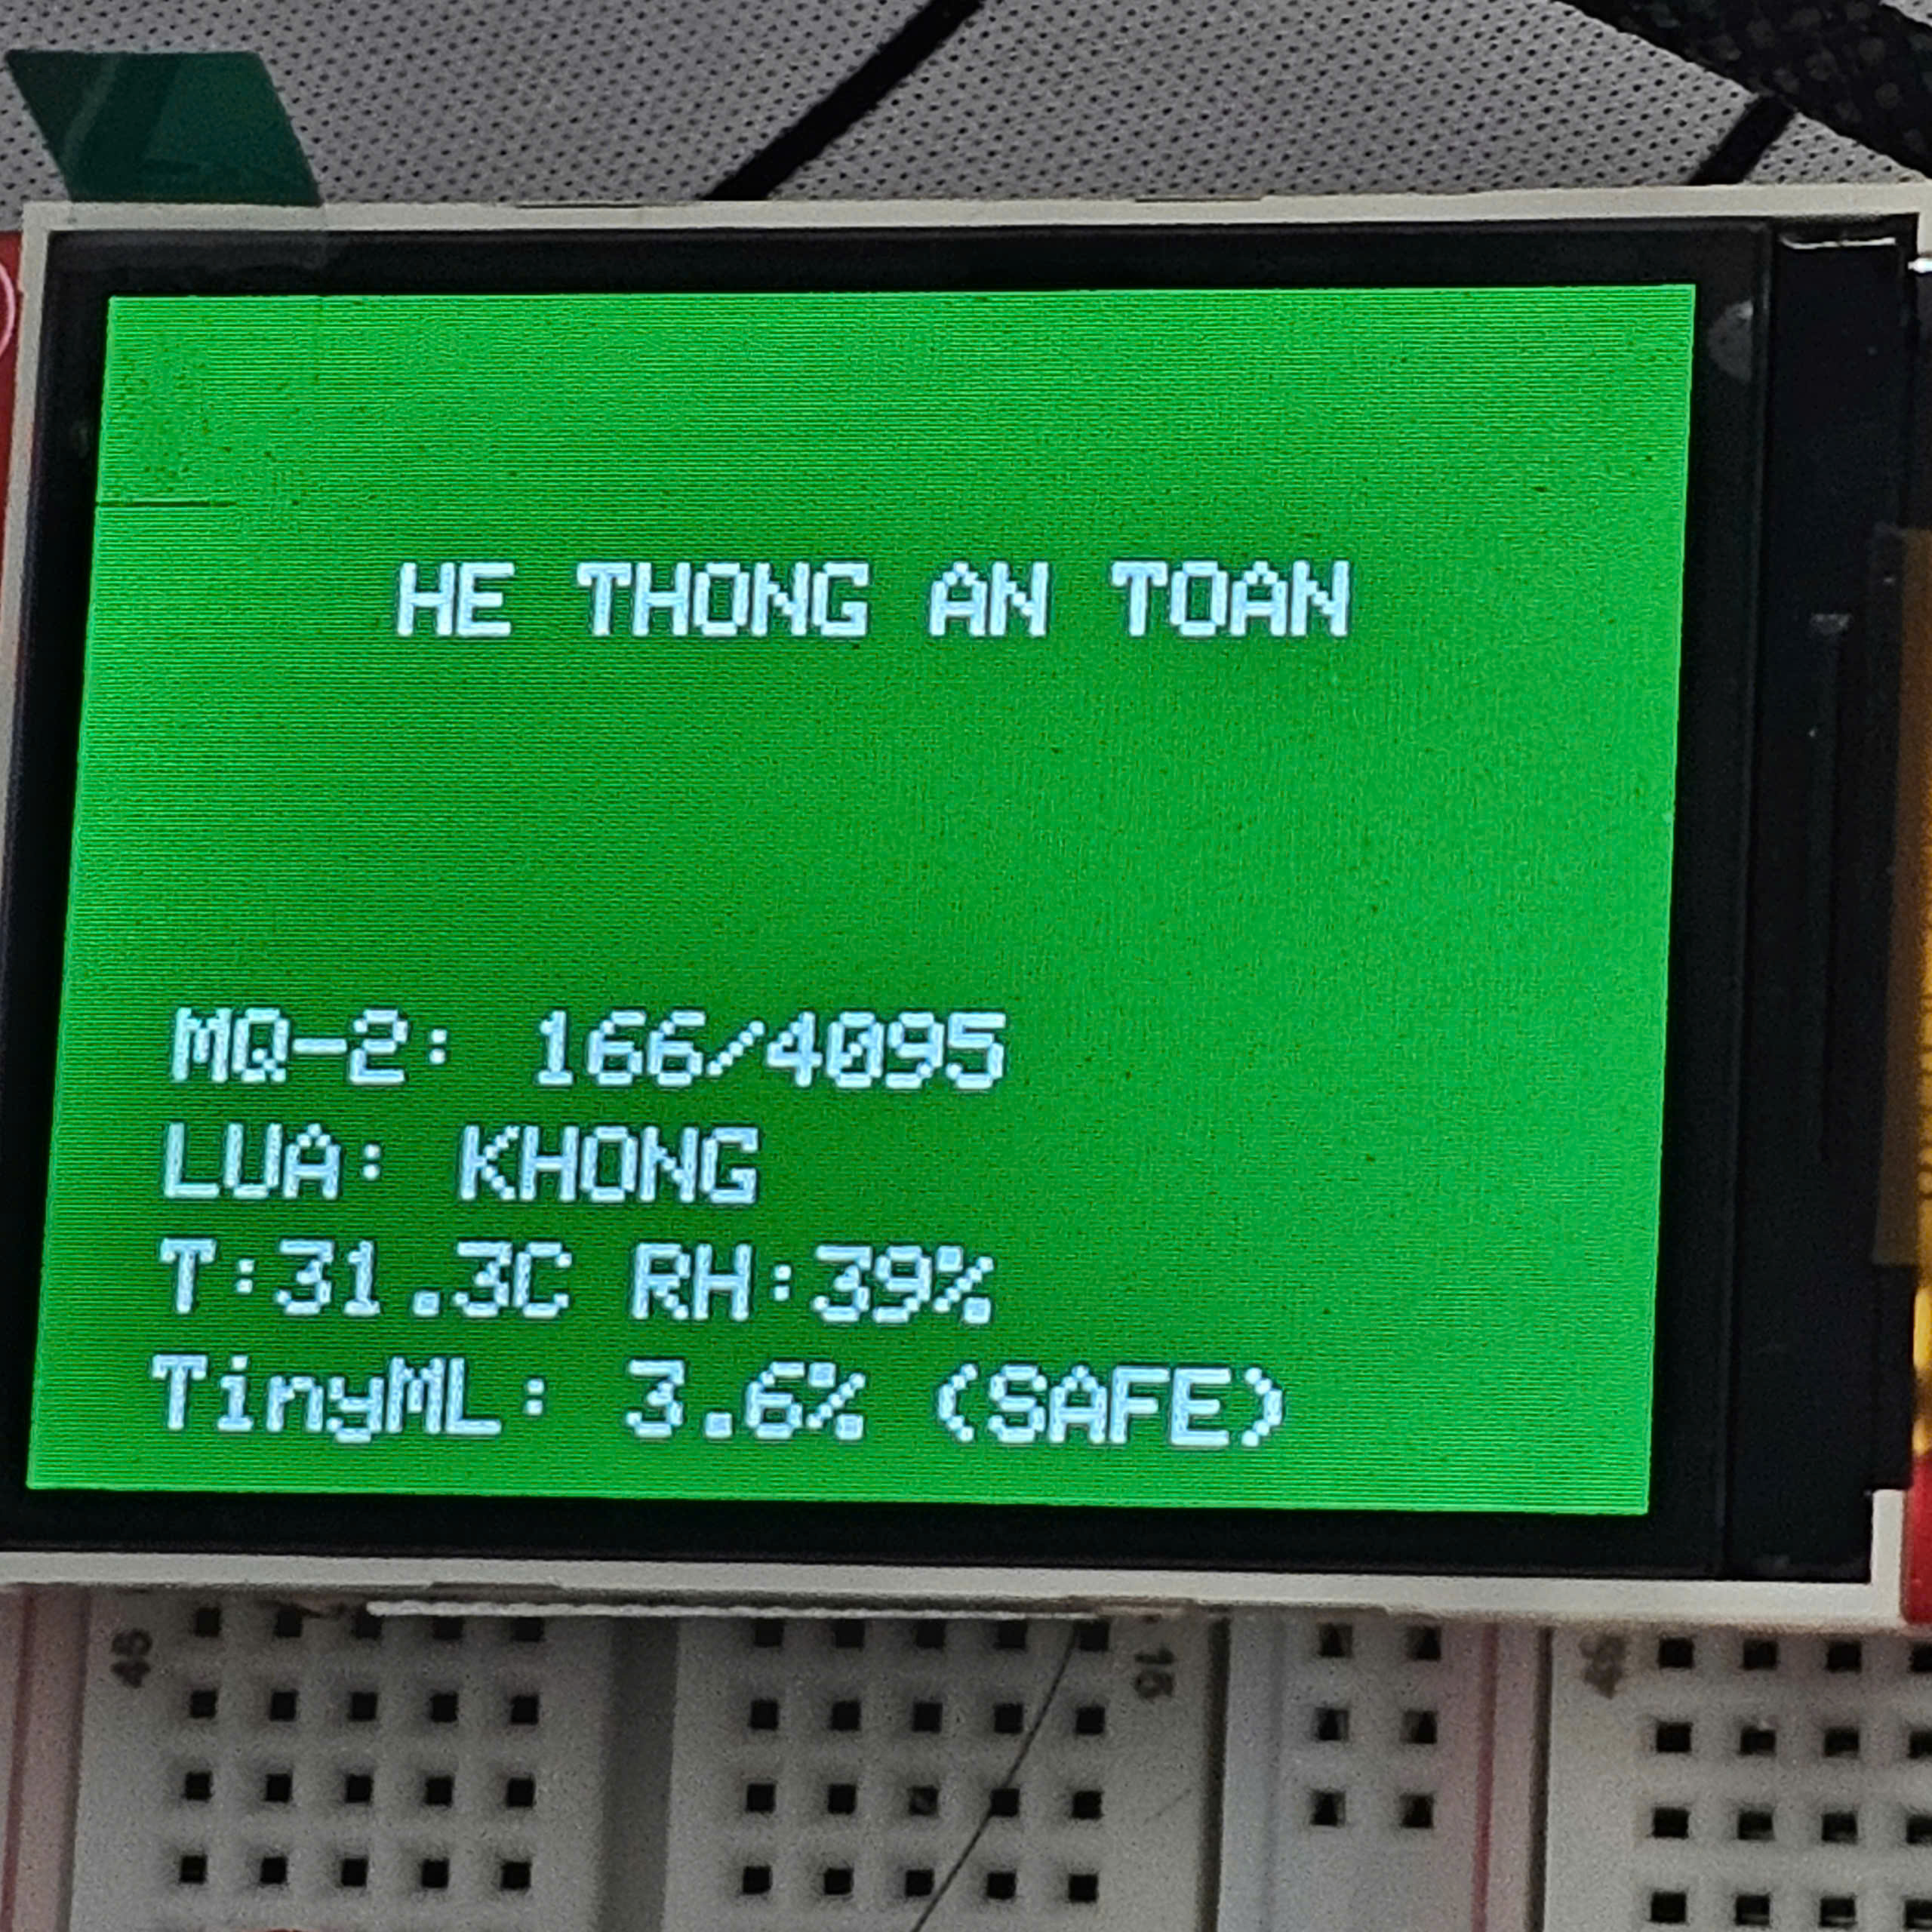
\includegraphics[width=\linewidth, height=6.0cm, keepaspectratio]{../../captured_picture/T04_1.jpg}
    \par\smallskip{\small (a) Trạng thái an toàn trên màn hình TFT (\texttt{T04\_1.jpg})}
  \end{minipage}
  \hfill
  \begin{minipage}[t]{0.48\textwidth}
    \centering
    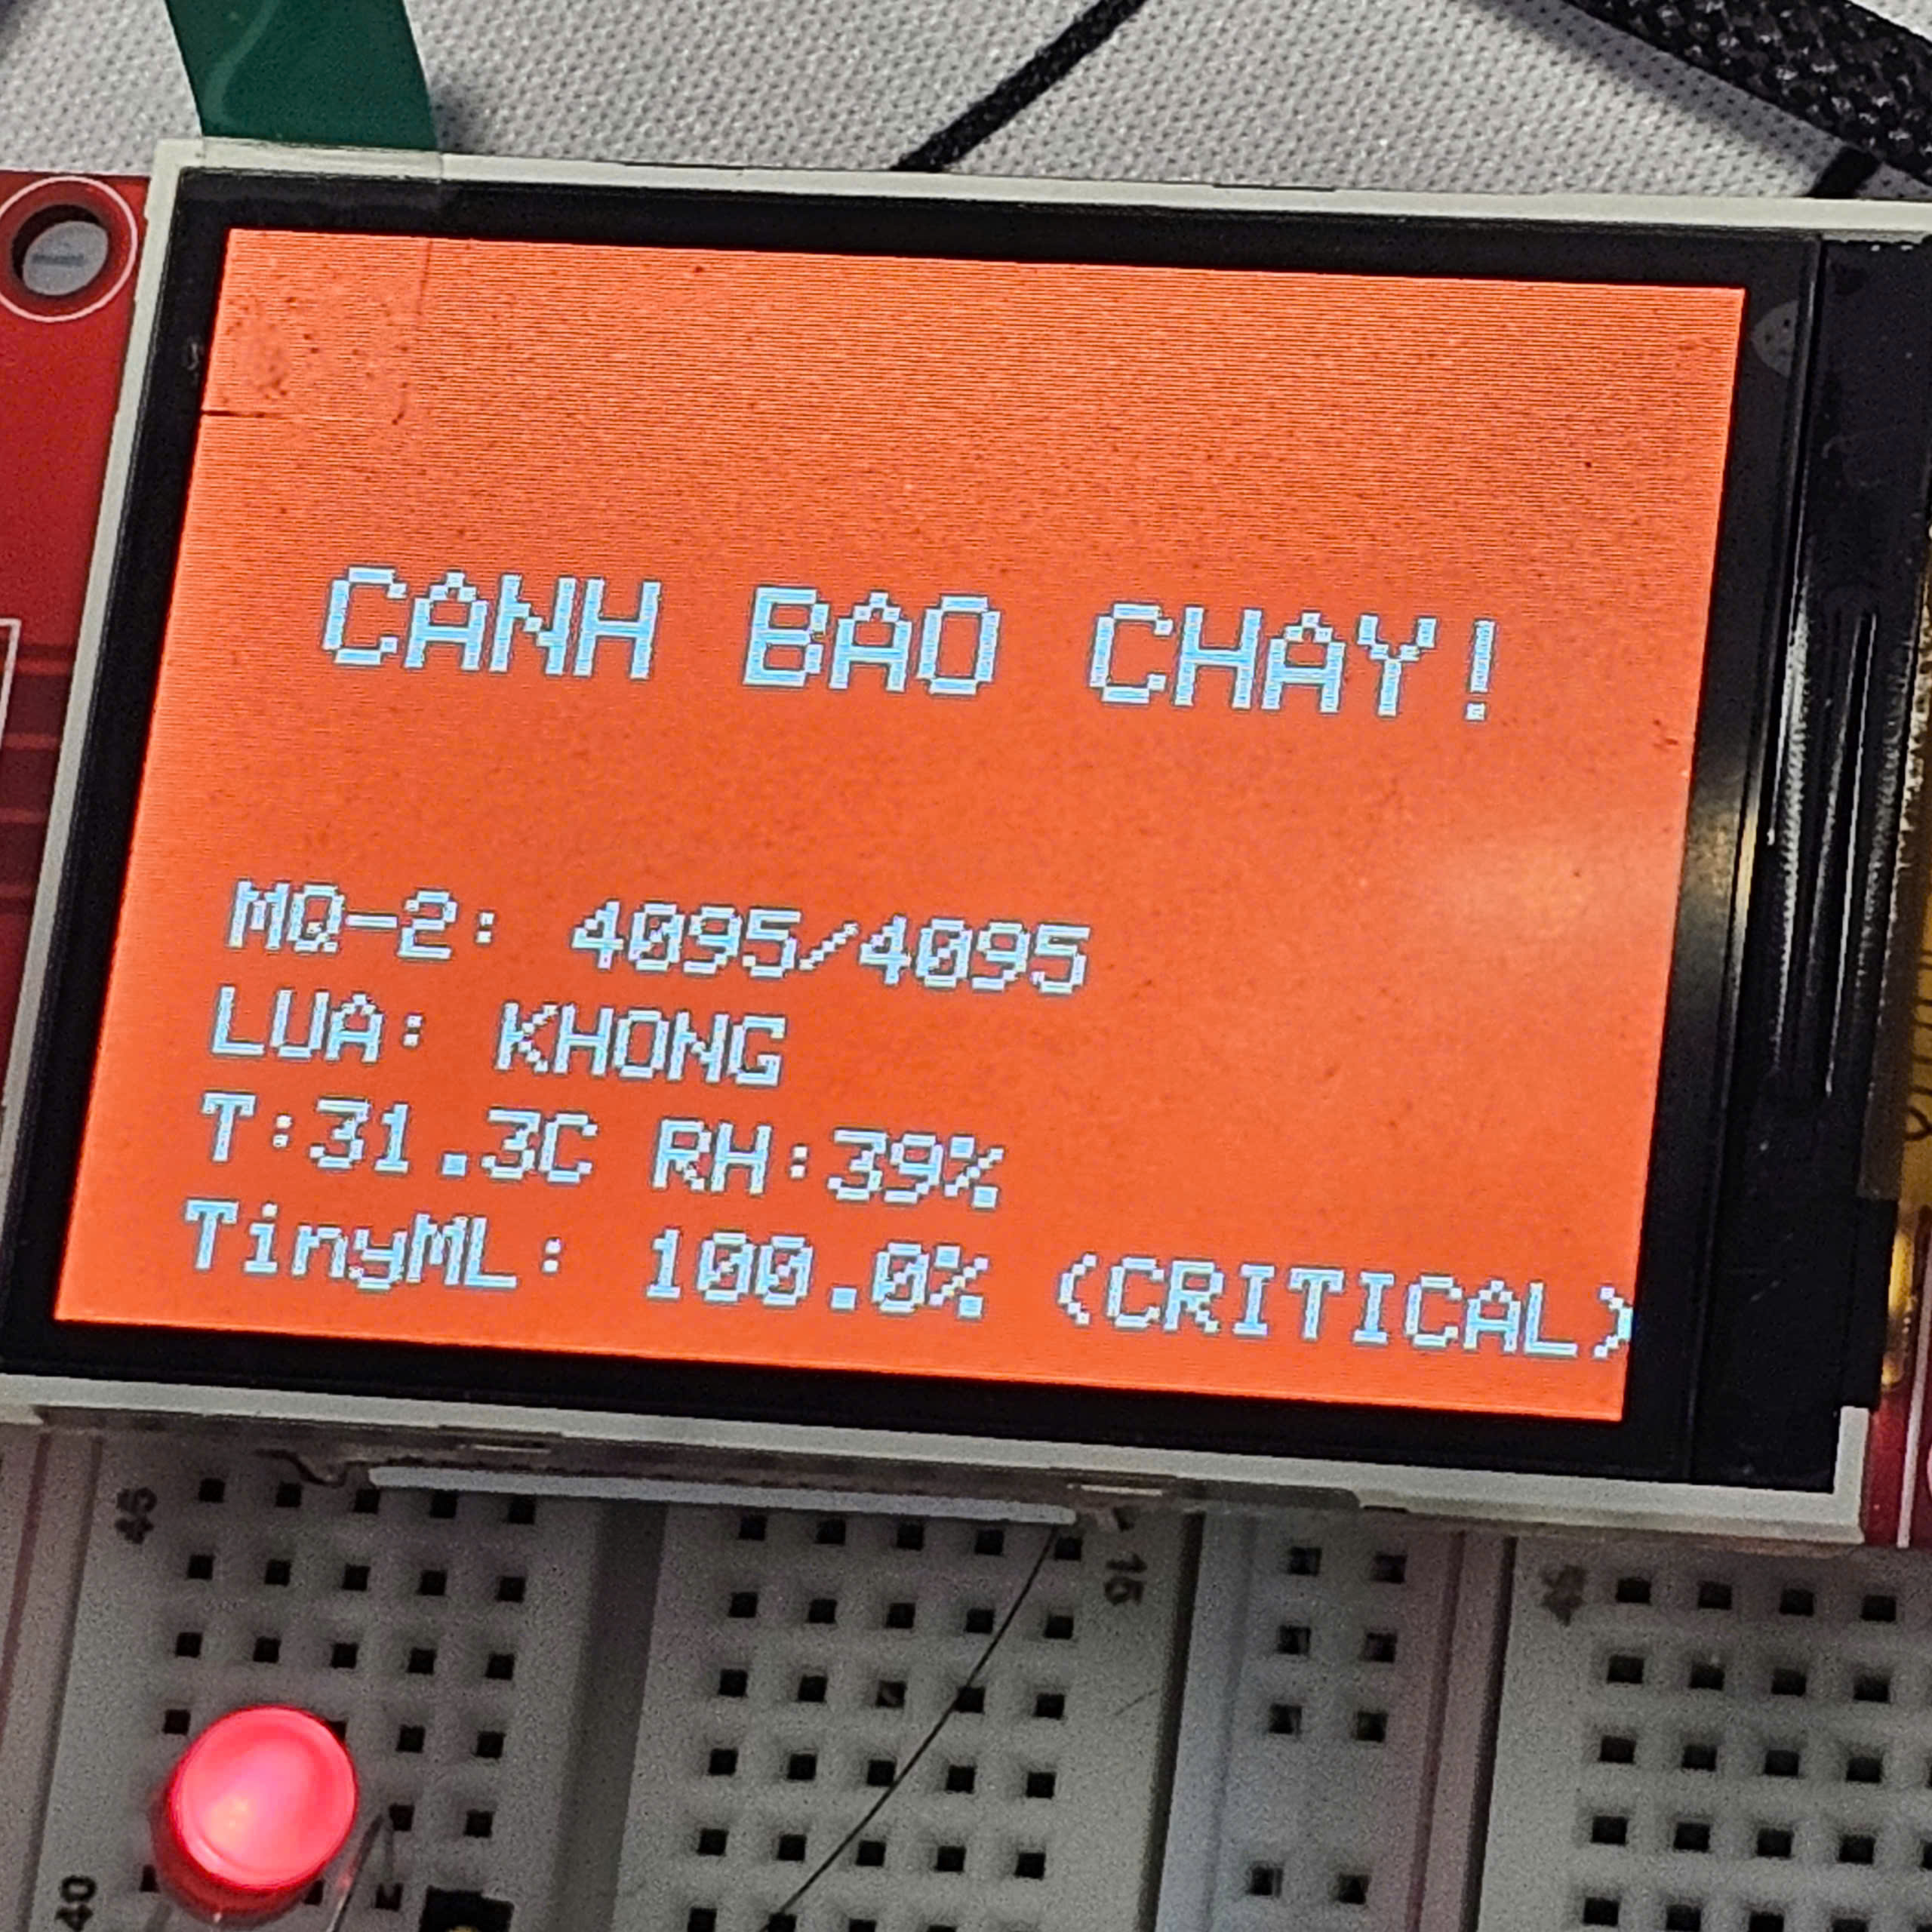
\includegraphics[width=\linewidth, height=6.0cm, keepaspectratio]{../../captured_picture/T04_2.jpg}
    \par\smallskip{\small (b) Trạng thái cảnh báo cháy trên màn hình TFT (\texttt{T04\_2.jpg})}
  \end{minipage}
  \caption{Hình ảnh phần cứng thực tế node YoloUNO ESP32-S3 và màn hình TFT ILI9341 ở hai trạng thái vận hành (T04)}
  \label{fig:so-do-dau-noi}
\end{figure}

\subsection{Firmware trên thiết bị}
\label{subsec:firmware-thiet-bi}

\subsubsection{Node cảm biến cháy và chấp hành YoloUNO (T04, T08)}
\label{subsubsec:node-1}

Firmware của End-Node được phát triển trên môi trường \textbf{PlatformIO} với cấu hình \texttt{[env:yolo\_uno]} trong tệp \texttt{01\_Firmware\_EndNode/platformio.ini}: nền tảng \texttt{espressif32}, bo mạch \texttt{esp32-s3-devkitc-1}, framework \texttt{arduino}, tốc độ Serial \texttt{115200} bps và cờ biên dịch \texttt{-D ARDUINO\_USB\_MODE=1}, \texttt{-D ARDUINO\_USB\_CDC\_ON\_BOOT=1}. Năm thư viện phụ thuộc gồm \texttt{Adafruit GFX Library}, \texttt{Adafruit ILI9341}, \texttt{ESP32Servo}, \texttt{DHT sensor library} và \texttt{Adafruit Unified Sensor}. Ngoài ra, thư mục \texttt{include/} có chuẩn bị sẵn tệp cấu hình \texttt{lv\_conf.h} (màu 16-bit, bộ nhớ đệm $32\text{ KB}$, bộ font Montserrat 12/14/32, giao diện tối) cho hướng mở rộng sang LVGL sau này; tuy nhiên ở phiên bản hiện thực chính thức, firmware điều khiển màn hình TFT ILI9341 trực tiếp bằng \texttt{Adafruit\_ILI9341} để tối ưu tốc độ vẽ lại màn hình và dung lượng Flash (vì vậy nhóm không khai báo tiêu chí \texttt{N03}).

Thay vì sử dụng hàm \texttt{delay()} gây nghẽn, vòng lặp \texttt{loop()} vận hành theo kiến trúc định thời không chặn (non-blocking cooperative scheduling) dựa trên \texttt{millis()} với ba chu kỳ độc lập và các cơ chế an toàn quan trọng:
\begin{enumerate}[leftmargin=*, itemsep=2pt]
  \item \textbf{Xử lý lệnh UART liên tục:} Hàm \texttt{processSerialCommands()} đọc bộ đệm 128 byte không chặn ở mỗi vòng lặp, nhận diện lệnh \texttt{alarm\_override}, \texttt{servo}, \texttt{buzzer}, \texttt{led} (tương thích cả định dạng JSON rút gọn lẫn định dạng RPC của ThingsBoard).
  \item \textbf{Cơ chế trễ (Hysteresis) và ưu tiên an toàn tuyệt đối:} Cảm biến MQ-2 kích hoạt khi $\text{ADC} \ge 1800$ và chỉ xóa khi $\text{ADC} \le 1650$; nhiệt độ DHT11 kích hoạt khi $T \ge 35.0^\circ\text{C}$ và xóa khi $T \le 34.0^\circ\text{C}$; cảm biến lửa kích hoạt tức thì khi \texttt{FLAME\_PIN == LOW}. Khi nhận lệnh điều khiển thủ công từ xa, cờ \texttt{manualOverrideUntil} giữ trạng thái thủ công trong $5000\text{ ms}$, nhưng nếu cảm biến phát hiện cháy thật (\texttt{!nextSafe}), firmware lập tức đặt \texttt{manualOverrideUntil = 0} để ép thực thi quy trình cứu hỏa.
  \item \textbf{Hiệu chỉnh tỷ số truyền cơ khí Servo:} Do liên kết cơ khí giữa trục Servo và cánh cửa mô hình có hành trình thực bằng một nửa góc quay trục, hằng số \texttt{SERVO\_COMMAND\_SCALE = 2} tự động nhân đôi góc logic ($0^\circ$--$90^\circ$) nhận từ Gateway sang góc vật lý ($0^\circ$--$180^\circ$, giới hạn tối đa \texttt{SERVO\_CLOSED\_ANGLE = 180}).
\end{enumerate}

Đoạn mã \ref{lst:main-loop} trích lược logic lấy mẫu, suy luận TinyML và xuất bản tin telemetry tại lõi hàm \texttt{loop()} trong \texttt{01\_Firmware\_EndNode/src/main.cpp}.

\begin{lstlisting}[language=C++, caption={Logic lấy mẫu đa cảm biến, suy luận TinyML và báo cáo UART trong \texttt{main.cpp}}, label={lst:main-loop}]
if (static_cast<uint32_t>(now - lastSensorSample) >= SENSOR_SAMPLE_INTERVAL_MS) {
  lastSensorSample = now;
  const int mq2Value = analogRead(MQ2_PIN);
  const bool flameDetected = digitalRead(FLAME_PIN) == LOW;
  if (!mq2AlarmActive && mq2Value >= MQ2_ALARM_THRESHOLD) mq2AlarmActive = true;
  else if (mq2AlarmActive && mq2Value <= MQ2_CLEAR_THRESHOLD) mq2AlarmActive = false;

  const bool nextSafe = !mq2AlarmActive && !flameDetected && !temperatureAlarmActive;
  const float curTemp = isnan(temperatureC) ? 28.0f : temperatureC;
  const float curHum  = isnan(humidityPercent) ? 65.0f : humidityPercent;
  const float aiRisk  = tinyml_predict_fire_risk(
      static_cast<float>(mq2Value), curTemp, flameDetected ? 1.0f : 0.0f, curHum);

  if (nextSafe != showingSafe) {
    if (!nextSafe) manualOverrideUntil = 0; // Real danger overrides manual state
    if (!nextSafe || now >= manualOverrideUntil) {
      showingSafe = nextSafe;
      showStatus(showingSafe, mq2Value, flameDetected, temperatureC, humidityPercent, aiRisk);
    }
  }
  if (static_cast<uint32_t>(now - lastSerialReport) >= SERIAL_REPORT_INTERVAL_MS) {
    lastSerialReport = now;
    Serial.printf("MQ-2 ADC: %d | Lua: %s | Nhiet do: %.1f C | Do am: %.0f%% | "
                  "AI Risk: %.1f%% | Trang thai: %s\n",
                  mq2Value, flameDetected ? "PHAT HIEN" : "KHONG",
                  temperatureC, humidityPercent, aiRisk * 100.0f,
                  showingSafe ? "AN TOAN" : "CANH BAO");
  }
}
\end{lstlisting}

\subsubsection{Webserver trên thiết bị (T07)}
\label{subsubsec:webserver-thiet-bi}

Trong phiên bản hiện thực này, nhóm \textbf{không triển khai Webserver trực tiếp trên ESP32-S3 (T07)}. Thay vào đó, giao diện giám sát và điều khiển cục bộ được đặt tập trung tại máy chủ HTTP nhúng của Local IoT Gateway (cổng \texttt{5050}, tiêu chí \texttt{T10} và \texttt{N06}, trình bày tại Mục \ref{subsec:iot-gateway}). Lựa chọn kiến trúc này giúp giải phóng toàn bộ ngăn xếp mạng TCP/IP trên vi điều khiển, đảm bảo tính định thời cứng cho vòng lặp đọc cảm biến $100\text{ ms}$, vẽ màn hình TFT SPI và suy luận TinyML mà không xảy ra gián đoạn do truy cập HTTP đồng thời.

\subsection{Truyền thông giữa các thiết bị}
\label{subsec:truyen-thong-thiet-bi}

Hệ thống sử dụng mô hình kết nối trực tiếp \textbf{UART USB-CDC 115200 bps} giữa End-Node YoloUNO (ESP32-S3) và Local IoT Gateway trên PC (không sử dụng BLE -- T03 hay ESP-NOW -- T06). Luồng truyền thông hai chiều được quản lý bởi lớp \path{HardwareSerialAdapter} và hàm \path{parse_uart_payload()} trong \path{02_Local_Gateway/hardware_gateway/LocalGateway.py}:
\begin{itemize}[leftmargin=*, itemsep=2pt]
  \item \textbf{Chiều Uplink (ESP32-S3 $\rightarrow$ PC):} \texttt{HardwareSerialAdapter} tự động quét các cổng COM dựa trên mô tả phần cứng (\texttt{ESP32}, \texttt{CH340}, \texttt{CP210}, \texttt{UART}, \texttt{USB SERIAL}, \texttt{303A}), mở cổng với \texttt{timeout=1.0 s} và xóa bộ đệm đầu vào. Hàm \texttt{parse\_uart\_payload()} hỗ trợ phân tích đồng thời cả chuỗi JSON chuẩn lẫn định dạng văn bản từ \texttt{main.cpp} bằng biểu thức chính quy, trích xuất đầy đủ các trường \texttt{smoke}, \texttt{flame}, \texttt{temperature}, \texttt{humidity}, \texttt{tinyml\_risk} và \texttt{status}.
  \item \textbf{Chiều Downlink (PC $\rightarrow$ ESP32-S3):} Lệnh điều khiển từ Cloud RPC hoặc Web Monitor được đưa vào \texttt{queue.Queue} và tuần tự hóa thành JSON kết thúc bằng \texttt{\textbackslash n} qua \texttt{write\_command()} có khóa đồng bộ \texttt{threading.Lock}, đảm bảo không xảy ra xung đột luồng trên cổng nối tiếp.
\end{itemize}

Hình \ref{fig:uart-gateway-log} minh chứng nhật ký truyền nhận hai chiều thực tế giữa bo mạch ESP32-S3 và Local Gateway trên Terminal (tiêu chí \texttt{T08}).

\begin{figure}[H]
  \centering
  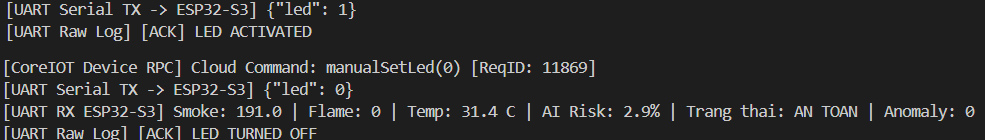
\includegraphics[width=0.92\textwidth]{../../captured_picture/T08.png}
  \caption{Minh chứng luồng truyền nhận UART hai chiều giữa ESP32-S3 và Local Gateway trên PC (T08 -- \texttt{T08.png})}
  \label{fig:uart-gateway-log}
\end{figure}

\subsection{IoT Gateway}
\label{subsec:iot-gateway}

Phân hệ Local IoT Gateway được xây dựng bằng Python 3 trong thư mục \path{02_Local_Gateway/} với các thư viện chính gồm \texttt{pyserial}, \texttt{paho-mqtt}, \texttt{scikit-learn}, \texttt{numpy} và các mô-đun chuẩn (\texttt{sqlite3}, \path{http.server}, \texttt{socketserver}, \texttt{threading}, \texttt{queue}). Hệ thống cung cấp các trình khởi chạy tự động gồm \path{run_system.py} (tại thư mục gốc), \path{02_Local_Gateway/run_hardware_gateway.py} và \path{02_Local_Gateway/start_system.py}, cho phép tự dò cổng COM, tự phát hiện container ThingsBoard cục bộ (cổng \texttt{1883}/\texttt{9090}), mở đồng thời hai bảng điều khiển trên trình duyệt và xử lý tín hiệu \texttt{SIGINT}/\texttt{SIGTERM} để giải phóng cổng COM an toàn khi nhấn \texttt{Ctrl+C}.

\textbf{Cơ chế lưu đệm ngoại tuyến SQLite WAL và đồng bộ Gateway (T08, T15):}
Lớp \path{OfflineBufferRepository} trong \path{02_Local_Gateway/ui/gateway_infrastructure.py} khởi tạo cơ sở dữ liệu \path{gateway_hardware_buffer.db} ở chế độ Write-Ahead Logging với lược đồ bảng:
\begin{center}
  \texttt{telemetry\_buffer(id INTEGER PRIMARY KEY AUTOINCREMENT, payload TEXT, timestamp REAL, synced INTEGER DEFAULT 0)}
\end{center}
Mỗi khi nhận bản tin mới từ UART, luồng chính tính toán kết quả Isolation Forest (\texttt{is\_anomaly}, \texttt{anomaly\_score}), sinh chuỗi \texttt{alarm\_status} và \texttt{alarm\_notification}, chèn ngay bản tin vào SQLite (\texttt{synced = 0}), rồi đẩy tức thời qua MQTT QoS 1 nếu kết nối đang khả dụng. Song song đó, luồng nền \texttt{sync\_worker} thức dậy mỗi $3.0\text{ s}$: khi cờ \texttt{cloud\_connected} chuyển sang \texttt{True}, tiến trình truy vấn tối đa 25 bản ghi chưa đồng bộ theo thứ tự FIFO, phát hành lên chủ đề \texttt{v1/devices/me/telemetry} (hoặc \texttt{v1/gateway/telemetry} cho thiết bị con \texttt{YOLOUNO\_FIRE\_NODE\_01} khi bật cờ \texttt{--gateway-api}), đánh dấu \texttt{synced = 1} khi nhận mã \texttt{MQTT\_ERR\_SUCCESS}, và dọn các bản ghi đã đồng bộ cũ hơn 7 ngày (\texttt{purge\_synced}).

\begin{lstlisting}[language=Python, caption={Luồng đồng bộ bù FIFO từ SQLite WAL lên CoreIOT/ThingsBoard trong \texttt{LocalGateway.py}}, label={lst:sync-worker}]
def sync_worker(self):
    while self.running:
        with self.telemetry_lock:
            cloud_ok = self.latest_telemetry["cloud_connected"]
            self.latest_telemetry["buffer_count"] = self.buffer_repo.count_unsynced()
        if cloud_ok:
            unsynced = self.buffer_repo.fetch_unsynced(limit=25)
            synced_ids = []
            for rec_id, payload_str in unsynced:
                if self.use_gateway_api:
                    rec_data = json.loads(payload_str)
                    gw_dev = "YOLOUNO_FIRE_NODE_01" if self.device_name == "FireAlarm_Gateway" else self.device_name
                    gw_msg = {gw_dev: [{"ts": int(time.time() * 1000), "values": rec_data}]}
                    info = self.mqtt_client.publish(GATEWAY_TELEMETRY_TOPIC, json.dumps(gw_msg), qos=1)
                else:
                    info = self.mqtt_client.publish(TELEMETRY_TOPIC, payload_str, qos=1)
                if info.rc == mqtt.MQTT_ERR_SUCCESS:
                    synced_ids.append(rec_id)
                else:
                    break
            if synced_ids:
                self.buffer_repo.mark_synced(synced_ids)
            self.buffer_repo.purge_synced(older_than_days=7.0)
        time.sleep(3.0)
\end{lstlisting}

\textbf{Giao diện giám sát -- điều khiển cục bộ SCADA (T10):}
Lớp \texttt{EmbeddedWebMonitor} phục vụ giao diện web chuẩn Keen Dashboards tại \texttt{http://localhost:5050}. Giao diện bao gồm thanh trạng thái trên cùng (chế độ Gateway, trạng thái kết nối CoreIOT Online/Offline Buffering, trạng thái End Node dựa trên chu kỳ kiểm tra $6\text{ s}$ và số bản ghi đang đệm trong SQLite), biểu ngữ cảnh báo cháy đỏ toàn chiều rộng, 5 thẻ thông số thời gian thực (Smoke Concentration ADC, Ambient Temperature, Flame Optical Sensor, Emergency Fire Door Servo, AI Isolation Forest), khu vực điều khiển cưỡng bức từng cơ cấu chấp hành kèm hai nút khẩn cấp (\texttt{TRIGGER EMERGENCY LOCKDOWN} và \texttt{RESTORE NORMAL OPERATION}). Hình \ref{fig:local-scada} trình bày giao diện hoạt động thực tế của Local SCADA Web Monitor.

\begin{figure}[H]
  \centering
  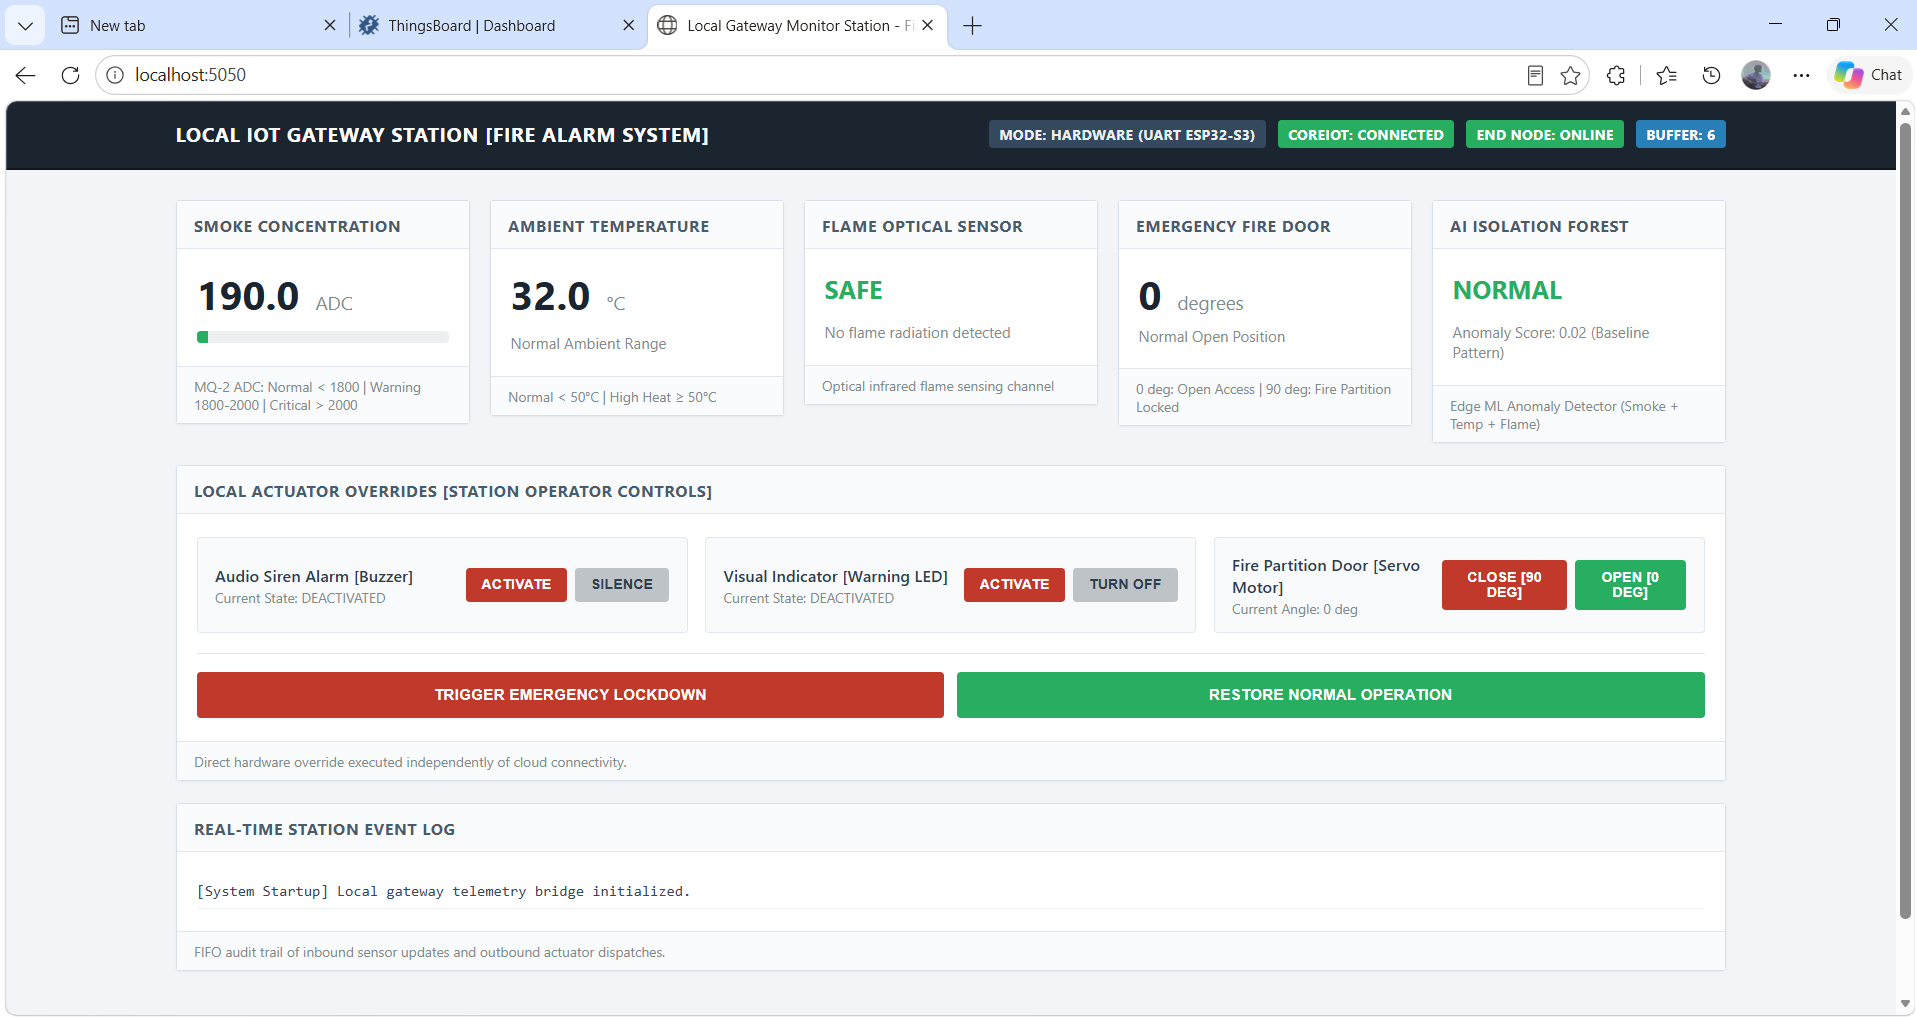
\includegraphics[width=0.95\textwidth]{../../captured_picture/T10.png}
  \caption{Giao diện giám sát và điều khiển SCADA cục bộ trên Local Gateway tại cổng 5050 (T10 -- \texttt{T10.png})}
  \label{fig:local-scada}
\end{figure}

\subsection{Trí tuệ nhân tạo}
\label{subsec:tri-tue-nhan-tao}

\subsubsection{Thu thập và chuẩn bị dữ liệu}
\label{subsubsec:ai-du-lieu}

Đối với mô hình TinyML trên vi điều khiển (tiêu chí \texttt{T05}), kịch bản \path{01_Firmware_EndNode/tinyml/train_tinyml.py} thực hiện tổng hợp tập dữ liệu đa chiều gồm \textbf{2.500 mẫu} (hàm \path{generate_synthetic_dataset()} với \texttt{num\_samples=2500}, \texttt{random\_state=42}) phản ánh đặc tính vật lý của ba cảm biến thực tế trên bo mạch, với 4 đặc trưng đầu vào (\path{MQ2_ADC}, \texttt{TEMPERATURE}, \texttt{HUMIDITY}, \texttt{FLAME}) và 2 lớp nhãn (0: \textit{Safe}, 1: \textit{Fire Hazard}):
\begin{itemize}[leftmargin=*, itemsep=2pt]
  \item \textbf{Lớp an toàn (Safe -- $65\%$, 1.625 mẫu):} $\text{MQ-2} \sim \mathcal{N}(180, 40^2)$ giới hạn $[80, 500]$, nhiệt độ $\sim \mathcal{N}(28.0, 3.0^2)$ trong $[20.0, 38.0]^\circ\text{C}$, độ ẩm $\sim \mathcal{N}(65.0, 8.0^2)$ trong $[40.0, 90.0]\%$, $\text{Flame} = 0$.
  \item \textbf{Lớp nguy cơ cháy (Fire Hazard -- $35\%$, 875 mẫu):} Phân bổ theo ba kịch bản cháy thực tế: (A) \textit{Cháy bùng có lửa} ($40\%$: $\text{MQ-2} \in [500, 2500]$, $T \in [32, 60]^\circ\text{C}$, $\text{RH} \in [20, 55]\%$, $\text{Flame}=1$); (B) \textit{Cháy sinh khói/gas đậm đặc} ($40\%$: $\text{MQ-2} \in [1800, 3800]$, $T \in [28, 50]^\circ\text{C}$, $\text{Flame} \in \{0,1\}$ với xác suất $0.7/0.3$); (C) \textit{Quá nhiệt cháy âm ỉ} ($20\%$: $\text{MQ-2} \in [900, 2200]$, $T \in [50, 68]^\circ\text{C}$, $\text{RH} \in [20, 45]\%$, $\text{Flame} \in \{0,1\}$ với xác suất $0.8/0.2$).
\end{itemize}

Tập dữ liệu được xáo trộn và tách theo tỉ lệ $80/20$ phân tầng (\texttt{stratify=y}): \textbf{2.000 mẫu huấn luyện} và \textbf{500 mẫu kiểm thử}. Các đặc trưng được chuẩn hóa Z-score sử dụng giá trị trung bình và độ lệch chuẩn tính hoàn toàn trên tập huấn luyện nhằm tránh rò rỉ dữ liệu.

Đối với mô hình Isolation Forest trên Local Gateway (tiêu chí \texttt{T09}), lớp \texttt{IsolationDetector} (\texttt{02\_Local\_Gateway/ui/isolation\_detector.py}) khởi tạo tập nền an toàn gồm 100 mẫu phủ toàn bộ dải vận hành dưới ngưỡng báo động ($\text{smoke} < 1800\text{ ADC}$, $T \in [15, 34]^\circ\text{C}$, $\text{flame}=0$) để tránh phụ thuộc vào độ lệch nền (offset) của từng cảm biến MQ-2, đồng thời duy trì hàng đợi cửa sổ trượt \texttt{deque(maxlen=200)} trong quá trình vận hành.

\subsubsection{Huấn luyện và đánh giá mô hình}
\label{subsubsec:ai-huan-luyen}

\textbf{Mô hình TinyML (T05):} Sử dụng \texttt{LogisticRegression(C=1.0, max\_iter=1000, random\_state=42)} từ \texttt{scikit-learn}. Trên tập kiểm thử 500 mẫu, mô hình đạt độ chính xác tổng thể \textbf{100.00\%} như thể hiện trong kết quả đầu ra của \texttt{train\_tinyml.py} (Hình \ref{fig:tinyml-train}) và bảng tham số trích xuất trực tiếp từ \texttt{tinyml\_fire\_model.h} tại Bảng \ref{tab:tham-so-tinyml}. Dấu của các trọng số hoàn toàn phù hợp quy luật vật lý: trọng số dương lớn cho khói MQ-2 ($+3.760794$), nhiệt độ ($+1.929540$) và lửa ($+1.876357$), trong khi trọng số âm cho độ ẩm ($-1.685517$) vì môi trường cháy thường khô nóng.

\begin{table}[H]
  \centering
  \caption{Tham số chuẩn hóa Z-score và trọng số mô hình TinyML trích xuất từ \texttt{tinyml\_fire\_model.h}}
  \label{tab:tham-so-tinyml}
  \renewcommand{\arraystretch}{1.25}
  \begin{tabularx}{\textwidth}{|L{0.26\textwidth}|C{0.22\textwidth}|C{0.22\textwidth}|C{0.22\textwidth}|}
    \hline
    \rowcolor{iotTableHead}
    \textbf{Đặc trưng đầu vào} & \textbf{Trung bình ($\mu_i$)} & \textbf{Độ lệch chuẩn ($\sigma_i$)} & \textbf{Trọng số ($w_i$)} \\
    \hline
    \texttt{MQ2\_ADC} (0--4095) & 826.217565 & 1007.851218 & $+3.760794$ \\
    \hline
    \texttt{TEMPERATURE} ($^\circ\text{C}$) & 34.104391 & 10.501738 & $+1.929540$ \\
    \hline
    \texttt{HUMIDITY} ($\%$) & 55.451318 & 15.155835 & $-1.685517$ \\
    \hline
    \texttt{FLAME} (0 hoặc 1) & 0.194500 & 0.395815 & $+1.876357$ \\
    \hline
    \multicolumn{3}{|l|}{\textbf{Hệ số tự do (\texttt{TINYML\_BIAS}):}} & $-1.230645$ \\
    \hline
  \end{tabularx}
\end{table}

\begin{figure}[H]
  \centering
  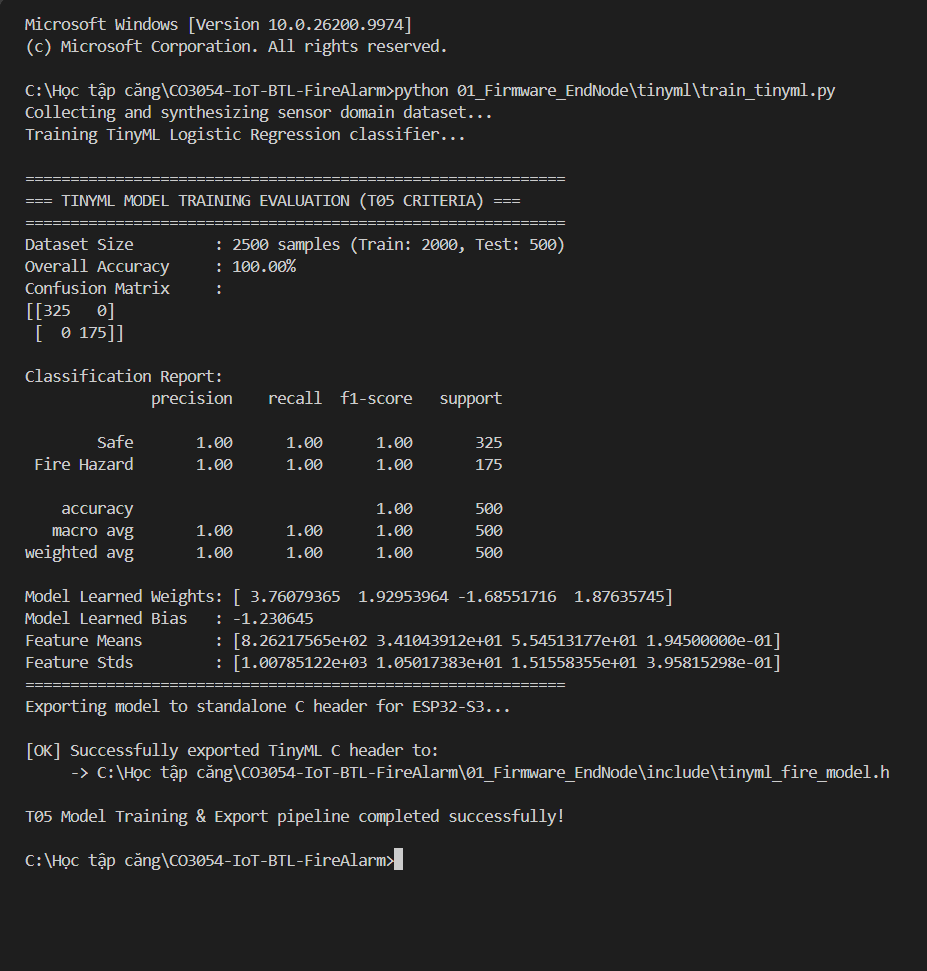
\includegraphics[width=0.9\textwidth]{../../captured_picture/T05.png}
  \caption[Kết quả huấn luyện TinyML và xuất tệp \texttt{tinyml\_fire\_model.h} (T05)]{Kết quả huấn luyện, đánh giá ma trận nhầm lẫn và xuất tệp \texttt{tinyml\_fire\_model.h} từ \texttt{train\_tinyml.py} (T05 -- \texttt{T05.png})}
  \label{fig:tinyml-train}
\end{figure}

\textbf{Mô hình Isolation Forest trên Local Gateway (T09):} Sử dụng thuật toán \texttt{IsolationForest} với siêu tham số \path{n_estimators=100}, \path{contamination=0.05} và \path{random_state=42}. Khi nhận mẫu đầu vào $[s, t, f]$, hệ thống kiểm tra tính hữu hạn (\path{math.isfinite}) để tránh lỗi \texttt{NaN}/\texttt{Inf} khi cảm biến đang làm nóng, đánh giá điều kiện bất thường cứng khớp ngưỡng firmware ($f > 0.5$ hoặc $s \ge 1800$ hoặc $t \ge 35.0^\circ\text{C}$), tính điểm \path{anomaly_score} theo phương trình \eqref{eq:iforest-score} và gán cờ \path{is_anomaly = 1} khi bộ dự đoán trả về $-1$, \path{anomaly_score >= 0.65} hoặc thỏa điều kiện cứng (khi đó điểm được nâng tối thiểu lên $0.90$). Hình \ref{fig:isolation-forest} minh chứng kết quả phát hiện thời gian thực trên Local Gateway ở hai trạng thái \texttt{NORMAL} và \texttt{ANOMALY DETECTED}.

\begin{figure}[H]
  \centering
  \begin{minipage}[t]{0.48\textwidth}
    \centering
    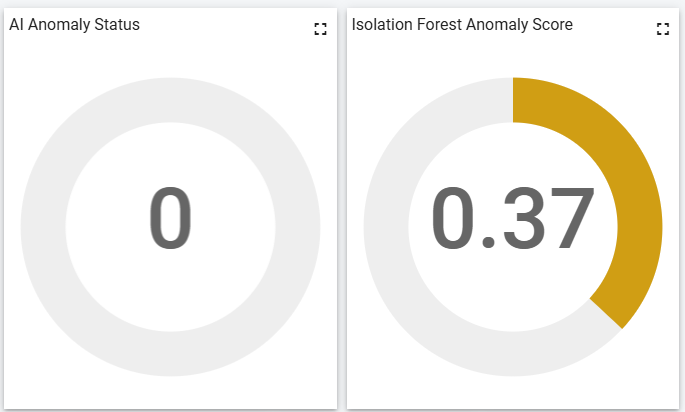
\includegraphics[width=\linewidth, height=4.8cm, keepaspectratio]{../../captured_picture/T09_1.png}
    \par\smallskip{\small (a) Trạng thái bình thường (\texttt{T09\_1.png})}
  \end{minipage}
  \hfill
  \begin{minipage}[t]{0.48\textwidth}
    \centering
    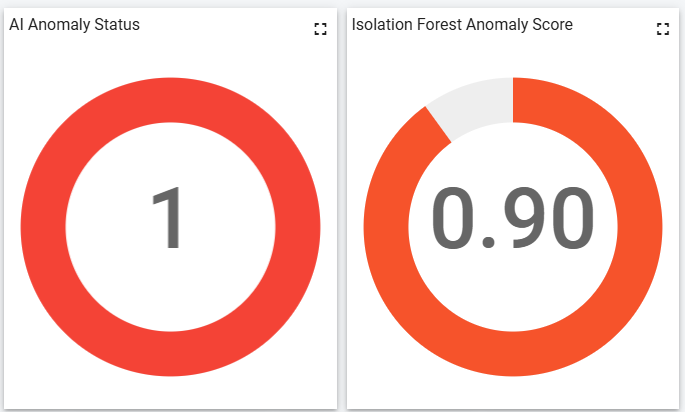
\includegraphics[width=\linewidth, height=4.8cm, keepaspectratio]{../../captured_picture/T09_2.png}
    \par\smallskip{\small (b) Phát hiện bất thường cháy (\texttt{T09\_2.png})}
  \end{minipage}
  \caption{Kết quả suy luận phát hiện bất thường đa biến bằng Isolation Forest trên Local Gateway (T09)}
  \label{fig:isolation-forest}
\end{figure}

\subsubsection{Triển khai mô hình}
\label{subsubsec:ai-trien-khai}

Hàm \path{export_c_header()} trong \path{train_tinyml.py} sinh trực tiếp tệp \path{01_Firmware_EndNode/include/tinyml_fire_model.h} gồm các hằng số mảng \texttt{static const float} và ba hàm nội tuyến \texttt{static inline}: \path{tinyml_sigmoid(float z)} (có chặn bão hòa tại $z > 12.0$ và $z < -12.0$ tránh tràn số), \path{tinyml_predict_fire_risk()} và \path{tinyml_get_risk_label()} phân chia ngưỡng rủi ro: $\ge 0.70 \rightarrow \texttt{CRITICAL}$, $\ge 0.40 \rightarrow \texttt{WARNING}$, $< 0.40 \rightarrow \texttt{SAFE}$.

Mô hình có dung lượng bộ nhớ ước tính chỉ khoảng \textbf{128 byte RAM}, hoàn toàn không sử dụng bộ nhớ động (zero heap allocation), được nhúng qua chỉ thị \texttt{\#include "tinyml\_fire\_model.h"} trong \texttt{main.cpp}. Kết quả xác suất cháy được hiển thị đồng thời trên dòng thứ 4 màn hình TFT ILI9341 (Hình \ref{fig:so-do-dau-noi}) và truyền lên Gateway qua trường \texttt{AI Risk} trong chuỗi Serial (Hình \ref{fig:tinyml-serial}).

\begin{figure}[H]
  \centering
  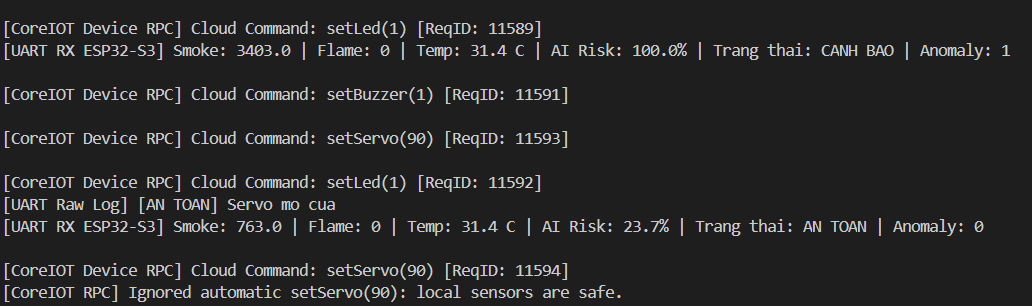
\includegraphics[width=0.92\textwidth]{../../captured_picture/T04_3.png}
  \caption{Minh chứng nhật ký Serial hiển thị xác suất rủi ro cháy \texttt{AI Risk} suy luận trực tiếp bởi TinyML trên ESP32-S3 (T04 -- \texttt{T04\_3.png})}
  \label{fig:tinyml-serial}
\end{figure}

\subsection{Nền tảng CoreIOT}
\label{subsec:nen-tang-coreiot}

\subsubsection{Device profile, template và dashboard (T11)}
\label{subsubsec:coreiot-dashboard}

Thay vì cấu hình thủ công trên giao diện web, nhóm xây dựng công cụ cấp phát tự động \path{02_Local_Gateway/dashboard/setup_thingsboard_dashboard.py}. Script thực hiện tuần tự 4 bước qua REST API của ThingsBoard: (1) chờ Spring Boot khởi động hoàn tất (timeout $180\text{ s}$); (2) đăng nhập tài khoản Tenant (\path{tenant@thingsboard.org}) để nhận mã JWT; (3) tạo hoặc truy xuất thiết bị \path{FireAlarm_Gateway} với \texttt{type = "Gateway"}, cờ \path{additionalInfo.gateway = true} và gán mã xác thực \path{i2tchqq1390qcxhun4zr}; (4) truy vấn các template widget hệ thống chuẩn của ThingsBoard 3.x, lắp ghép thành bảng điều khiển \textit{Industrial Fire Alarm \& Suppression System} gồm \textbf{10 widget} trên lưới 24 cột (cửa sổ thời gian thực 5 phút, chu kỳ $1\text{ s}$) và xuất lược đồ ra tệp \path{thingsboard_dashboard.json}. Danh sách chi tiết 10 widget được tổng hợp ở Bảng \ref{tab:tb-widgets} và ảnh chụp thực tế tại Hình \ref{fig:tb-dashboard}.

\begin{table}[htbp]
  \centering
  \caption[Cấu hình 10 widget trên ThingsBoard Industrial Dashboard]{Cấu hình 10 widget trên ThingsBoard Industrial Dashboard (\texttt{thingsboard\_dashboard.json})}
  \label{tab:tb-widgets}
  \renewcommand{\arraystretch}{1.22}
  \begin{tabularx}{\textwidth}{|C{0.05\textwidth}|L{0.25\textwidth}|L{0.23\textwidth}|C{0.14\textwidth}|Y|}
    \hline
    \rowcolor{iotTableHead}
    \textbf{STT} & \textbf{Tên Widget} & \textbf{Loại Widget (FQN)} & \textbf{Vị trí (r,c,w$\times$h)} & \textbf{Khóa dữ liệu / RPC} \\
    \hline
    1 & MQ-2 Raw ADC & Radial Gauge & (0,0, 5$\times$6) & \texttt{smoke} ($0$--$4095$; xanh $<1800$, cam $1800$--$2000$, đỏ $>2000$) \\
    \hline
    2 & Flame Detector Status & Digital Simple Gauge & (0,5, 5$\times$6) & \texttt{flame} ($0$: xanh, $1$: đỏ) \\
    \hline
    3 & Ambient Temperature & Value Card & (0,10, 4$\times$6) & \texttt{temperature} ($^\circ\text{C}$, icon nhiệt kế) \\
    \hline
    4 & AI Anomaly Status & Digital Simple Gauge & (0,14, 5$\times$6) & \texttt{is\_anomaly} ($0$ hoặc $1$) \\
    \hline
    5 & Isolation Forest Anomaly Score & Digital Simple Gauge & (0,19, 5$\times$6) & \texttt{anomaly\_score} ($0.00$--$1.00$) \\
    \hline
    6 & Environmental Telemetry History & Timeseries Chart & (6,0, 15$\times$7) & 4 kênh: \texttt{smoke}, \texttt{temperature}, \texttt{flame}, \texttt{anomaly\_score} \\
    \hline
    7 & Master Alarm Override & Round Switch (RPC) & (6,15, 3$\times$7) & \texttt{getAlarmOverride} / \texttt{setAlarmOverride} \\
    \hline
    8 & Alarm Siren Buzzer & Switch Control (RPC) & (6,18, 3$\times$7) & \texttt{getBuzzer} / \texttt{manualSetBuzzer} \\
    \hline
    9 & Strobe LED Beacon & Switch Control (RPC) & (6,21, 3$\times$7) & \texttt{getLed} / \texttt{manualSetLed} \\
    \hline
    10 & T13: Emergency Alarm Notification & Value Card & (13,0, 24$\times$3) & \texttt{alarm\_notification} (thanh cảnh báo toàn màn hình) \\
    \hline
  \end{tabularx}
\end{table}

\begin{figure}[H]
  \centering
  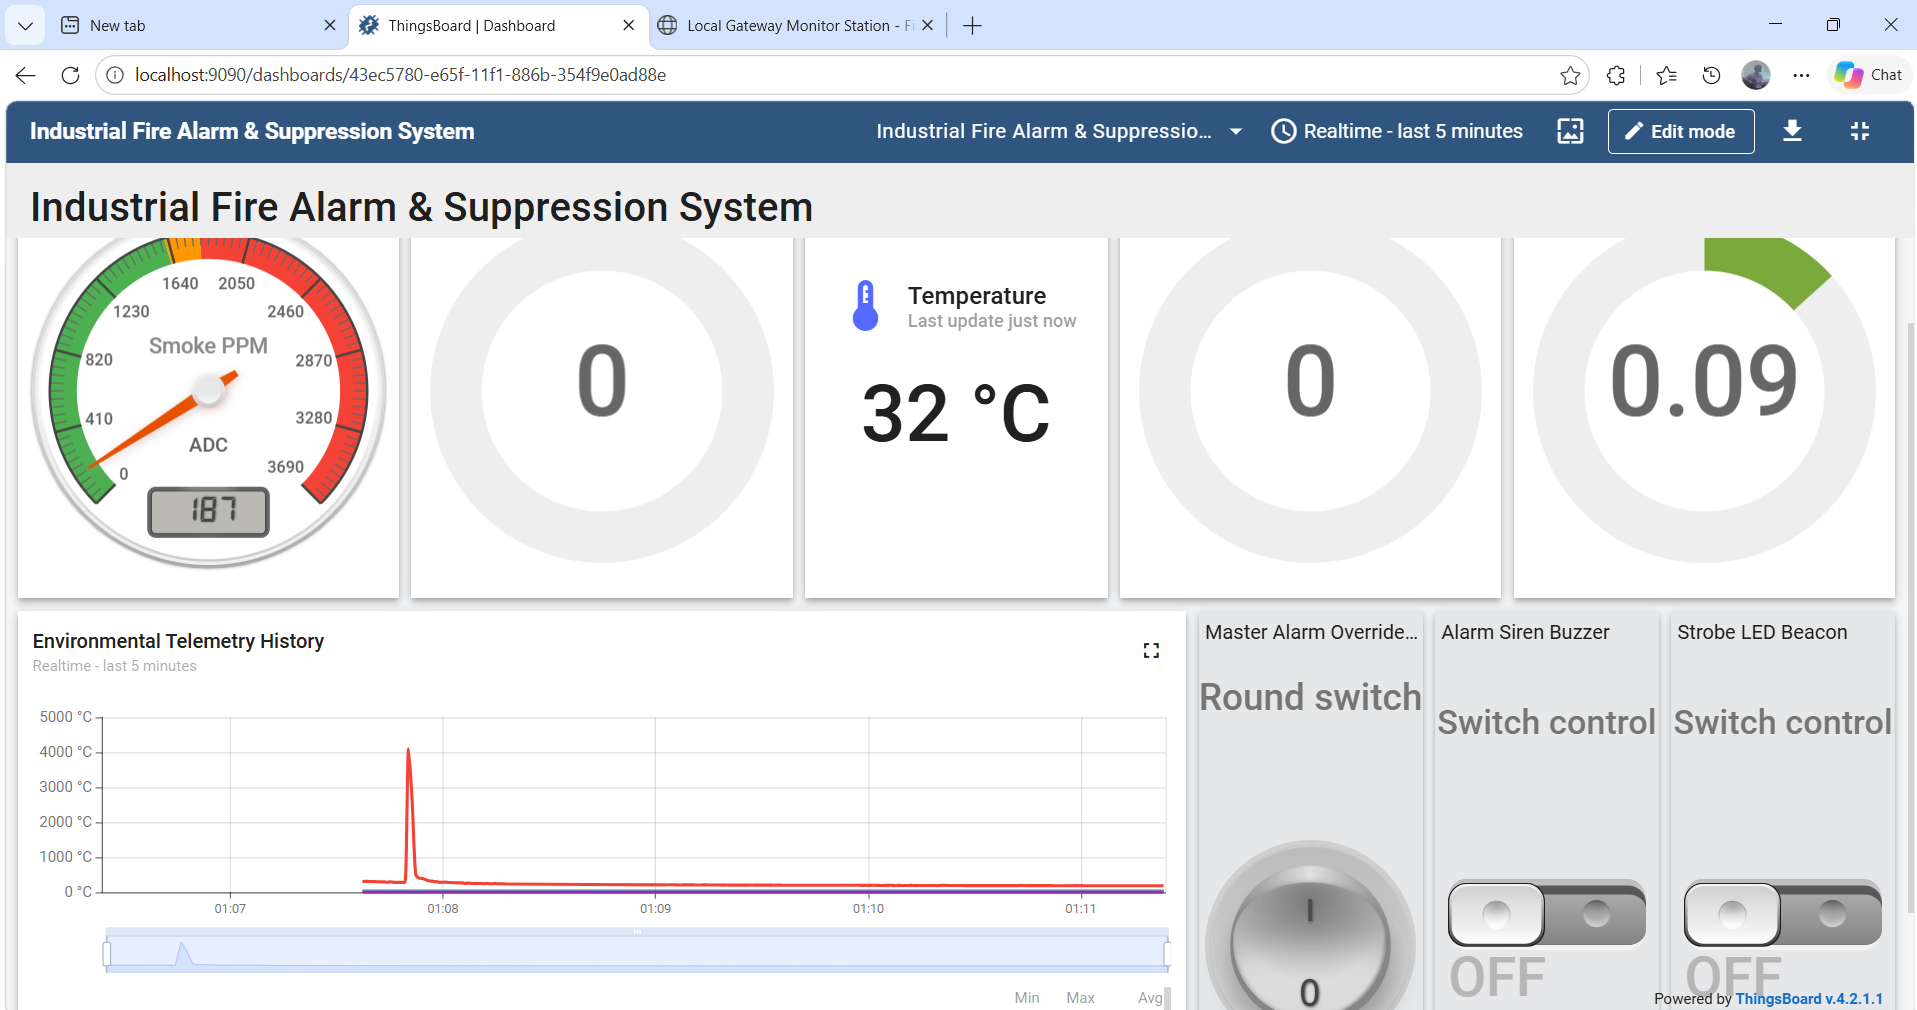
\includegraphics[width=0.96\textwidth]{../../captured_picture/T11.png}
  \caption{Giao diện Industrial Fire Alarm Dashboard với 10 widget giám sát, điều khiển RPC và Notification trên ThingsBoard (T11, T13 -- \texttt{T11.png})}
  \label{fig:tb-dashboard}
\end{figure}

\subsubsection{RuleChain (T12) và cảnh báo notification (T13)}
\label{subsubsec:coreiot-rulechain}

Luồng xử lý tự động phía máy chủ được định nghĩa chuẩn hóa trong \path{03_CoreIOT_Config/rule_chains/fire_alarm_rule_chain.json} và triển khai hai bước (\path{POST /api/ruleChain} và \path{POST /api/ruleChain/metadata}) thông qua kịch bản \path{03_CoreIOT_Config/scripts/setup_rule_chain.py}. Trong cấu hình JSON chuẩn, Rule Chain gồm 5 nút xử lý và 4 liên kết:
\begin{enumerate}[leftmargin=*, itemsep=2pt]
  \item \textbf{Filter Telemetry (\texttt{TbJsFilterNode}):} Kiểm tra sự tồn tại của các khóa telemetry liên quan đến cháy (\texttt{temperature}, \texttt{smoke\_level}, \texttt{tinyml\_fire}); nếu hợp lệ sẽ rẽ nhánh song song sang lưu chuỗi thời gian và đánh giá nguy cơ.
  \item \textbf{Save Telemetry (\texttt{TbMsgTimeseriesNode}):} Ghi bền vững dữ liệu chuỗi thời gian vào cơ sở dữ liệu PostgreSQL (\texttt{defaultTTL = 0}).
  \item \textbf{Evaluate Fire Risk (\texttt{TbJsSwitchNode}):} So sánh ngưỡng nhiệt độ ($> 50.0^\circ\text{C}$), ngưỡng khói ($> 400$) hoặc cờ suy luận TinyML (hỗ trợ ép kiểu đa dạng \texttt{true}, \texttt{1}, \texttt{'1'}, \texttt{'true'}) để rẽ nhánh \texttt{True} (nguy hiểm) hoặc \texttt{False} (bình thường).
  \item \textbf{Create Fire Alarm (\texttt{TbCreateAlarmNode}):} Tạo cảnh báo loại \texttt{FIRE\_ALARM} mức độ \texttt{CRITICAL}, đính kèm chi tiết cảm biến và bật \texttt{propagate = true}.
  \item \textbf{Clear Fire Alarm (\texttt{TbClearAlarmNode}):} Tự động xóa cảnh báo khi các thông số trở về trạng thái an toàn.
\end{enumerate}

Trên máy chủ ThingsBoard vận hành thực tế (Hình \ref{fig:tb-rulechain}), nhóm mở rộng nhánh xử lý của Rule Chain thành bộ phân loại 3 cấp độ (\texttt{Safe}, \texttt{Warning}, \texttt{Critical}) gắn trực tiếp với các nút \texttt{RPC Call Request} nhằm tự động phát đồng thời 3 lệnh điều khiển \texttt{setServo(90)}, \texttt{setBuzzer(1)} và \texttt{setLed(1)} xuống Gateway khi rơi vào nhánh \texttt{Critical}, và tự động đặt lại trạng thái khi trở về nhánh \texttt{Safe}.

\begin{figure}[H]
  \centering
  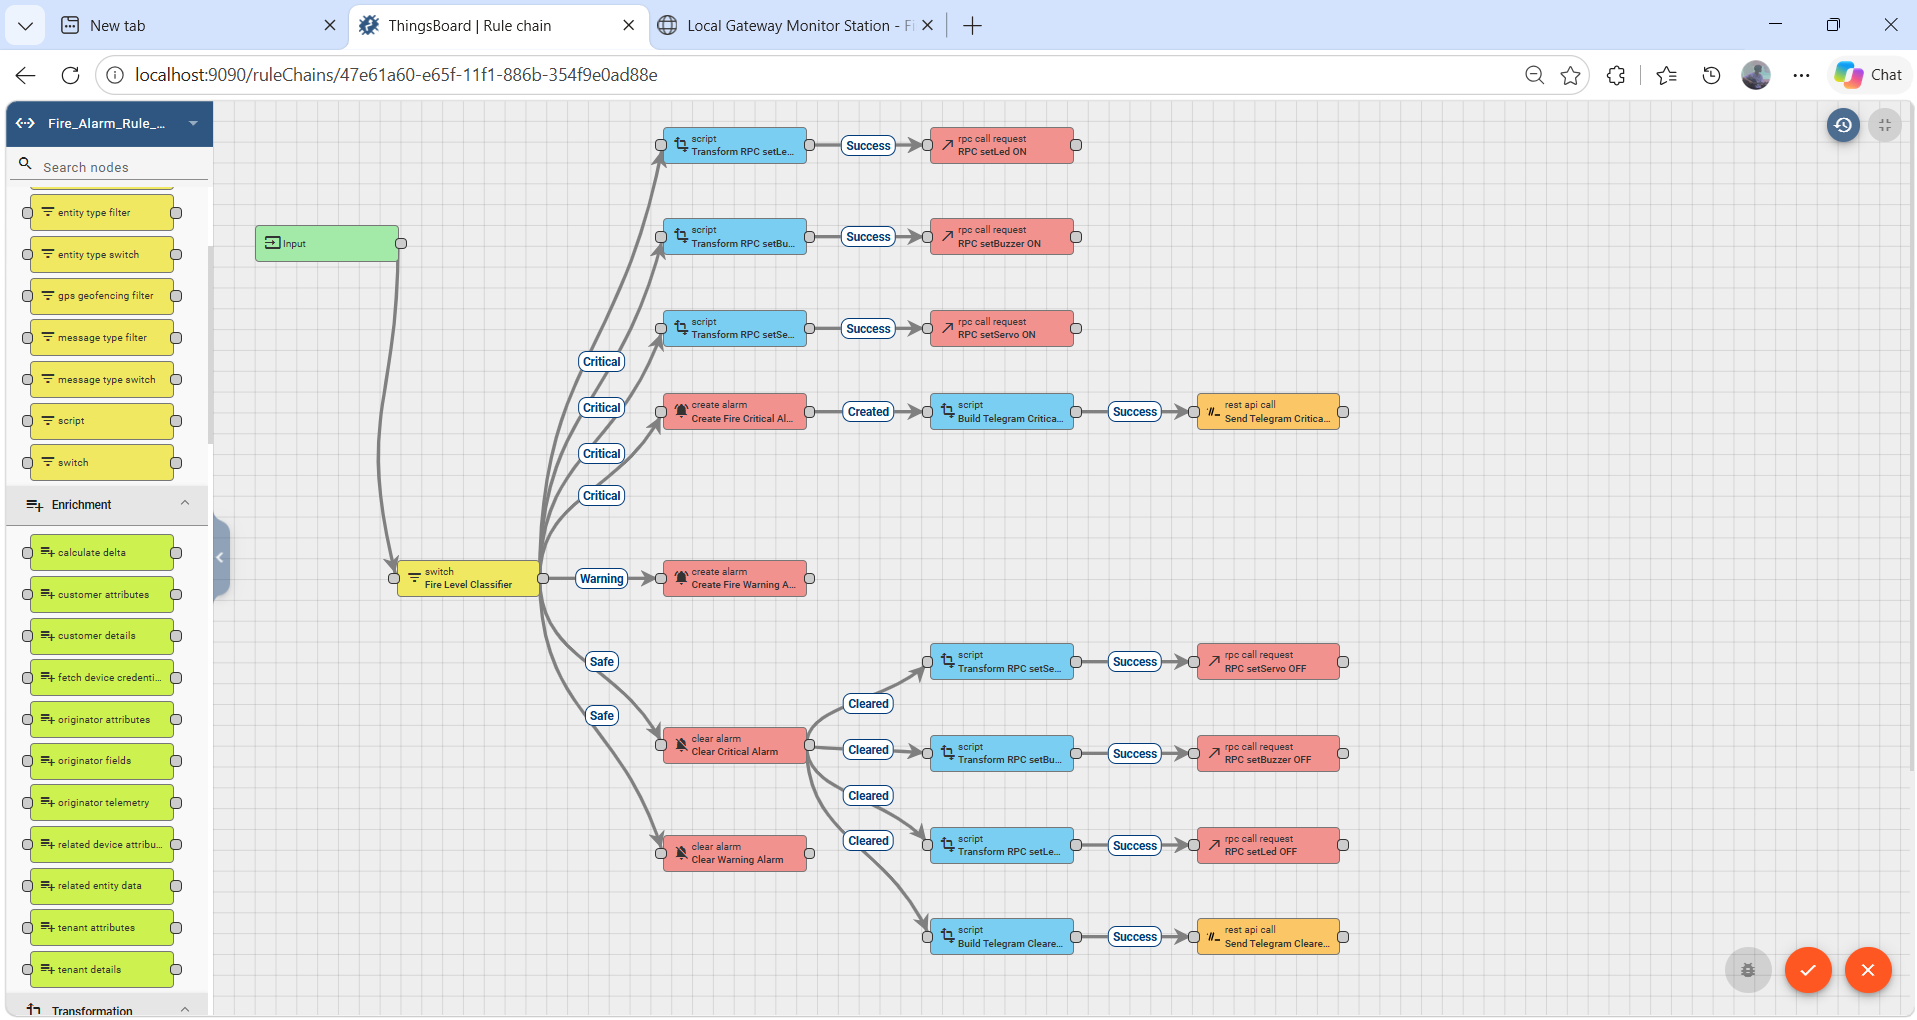
\includegraphics[width=0.95\textwidth]{../../captured_picture/T12.png}
  \caption{Sơ đồ Rule Chain xử lý phân loại nguy cơ cháy, quản lý Alarm và điều phối lệnh RPC trên ThingsBoard (T12 -- \texttt{T12.png})}
  \label{fig:tb-rulechain}
\end{figure}

Đối với tiêu chí \textbf{cảnh báo Notification (T13)}, hệ thống kết hợp tạo bản ghi Alarm gốc trên ThingsBoard với kênh thông báo thời gian thực trên giao diện Dashboard (Widget 10 -- \textit{T13: Emergency Alarm Notification (In-App Feed)}). Khi trạng thái cảm biến vượt ngưỡng, Local Gateway cập nhật chuỗi telemetry \path{alarm_notification} theo 3 mức: \textit{``[CRITICAL NOTIFICATION] Fire detected! Smoke: ... ADC, Temp: ...C. Auto lockdown active!''} (khi cháy), \textit{``[WARNING NOTIFICATION] Smoke elevating (... ADC)''} (khi khói $\ge 800\text{ ADC}$), và \textit{``[SAFE] System normal...''} (khi an toàn), giúp vận hành viên quan sát cảnh báo tức thời ngay trên màn hình trung tâm mà không phụ thuộc dịch vụ nhắn tin bên thứ ba.

\subsubsection{Cập nhật firmware OTA (T14)}
\label{subsubsec:coreiot-ota}

Tính năng cập nhật firmware từ xa OTA (\texttt{T14}) \textbf{chưa được hiện thực} trong phạm vi báo cáo này do End-Node giao tiếp với Local Gateway qua cổng nối tiếp USB-CDC thay vì duy trì phiên Wi-Fi/HTTP riêng biệt lên máy chủ CoreIOT. Việc nạp và nâng cấp firmware hiện được thực hiện trực tiếp qua công cụ PlatformIO (\texttt{pio run -e yolo\_uno -t upload}).

\subsection{Các tính năng nâng cao}
\label{subsec:tinh-nang-nang-cao}

Nhóm hiện thực thành công hai tính năng nâng cao có tổng điểm tích lũy $2.0$ (đạt trần tối đa $1.0/1.0$ điểm cộng):

\begin{enumerate}[leftmargin=*, itemsep=3pt]
  \item \textbf{Giao diện Dashboard tự thiết kế có khả năng phát hiện và ghi nhận sự kiện (N06):} Trên giao diện SCADA cục bộ (\path{02_Local_Gateway/ui/gateway_infrastructure.py}), bên cạnh 5 thẻ đo và bảng điều khiển chấp hành, nhóm xây dựng khu vực \textit{Real-Time Station Event Log} ghi nhận tự động theo hàng đợi FIFO (tối đa 25 sự kiện gần nhất) kèm dấu thời gian chính xác cho mọi thao tác phát lệnh chấp hành, kích hoạt phong tỏa khẩn cấp (\texttt{EMERGENCY}) và khôi phục trạng thái an toàn (\texttt{RESTORE}), kết hợp với biểu ngữ phát hiện cháy tự động (\path{#alert-banner}). Hình \ref{fig:n06-eventlog} minh họa bảng lưu vết sự kiện hoạt động thực tế.
  \item \textbf{Tự triển khai máy chủ ThingsBoard cục bộ bằng Docker (N07):} Tệp \path{02_Local_Gateway/dashboard/docker-compose.yml} định nghĩa dịch vụ \texttt{tb-postgres} từ ảnh chính thức \path{thingsboard/tb-postgres:latest} (tên container \texttt{thingsboard-local}), ánh xạ cổng HTTP \texttt{9090}, MQTT \texttt{1883}, Edge \texttt{7070}, CoAP \texttt{5683--5688/udp} và gắn volume bền vững \texttt{tb-data}, \texttt{tb-logs}. Kịch bản \path{deploy_thingsboard.py} tự động kiểm tra Docker Engine, khởi chạy stack, thăm dò trang đăng nhập HTTP \texttt{200 OK} cùng cổng TCP \texttt{1883} (timeout $180\text{ s}$) và hỗ trợ dừng sạch qua cờ \texttt{--stop}. Hình \ref{fig:n07-docker} xác nhận container \texttt{thingsboard-local} đang chạy ổn định trên Docker Desktop.
\end{enumerate}

\begin{figure}[H]
  \centering
  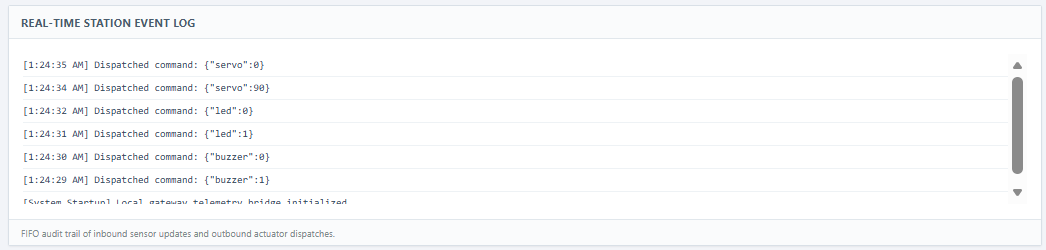
\includegraphics[width=0.92\textwidth]{../../captured_picture/N06.png}
  \caption{Bảng lưu vết sự kiện thời gian thực (Audit Trail Event Log) trên giao diện SCADA cục bộ (N06 -- \texttt{N06.png})}
  \label{fig:n06-eventlog}
\end{figure}

\begin{figure}[H]
  \centering
  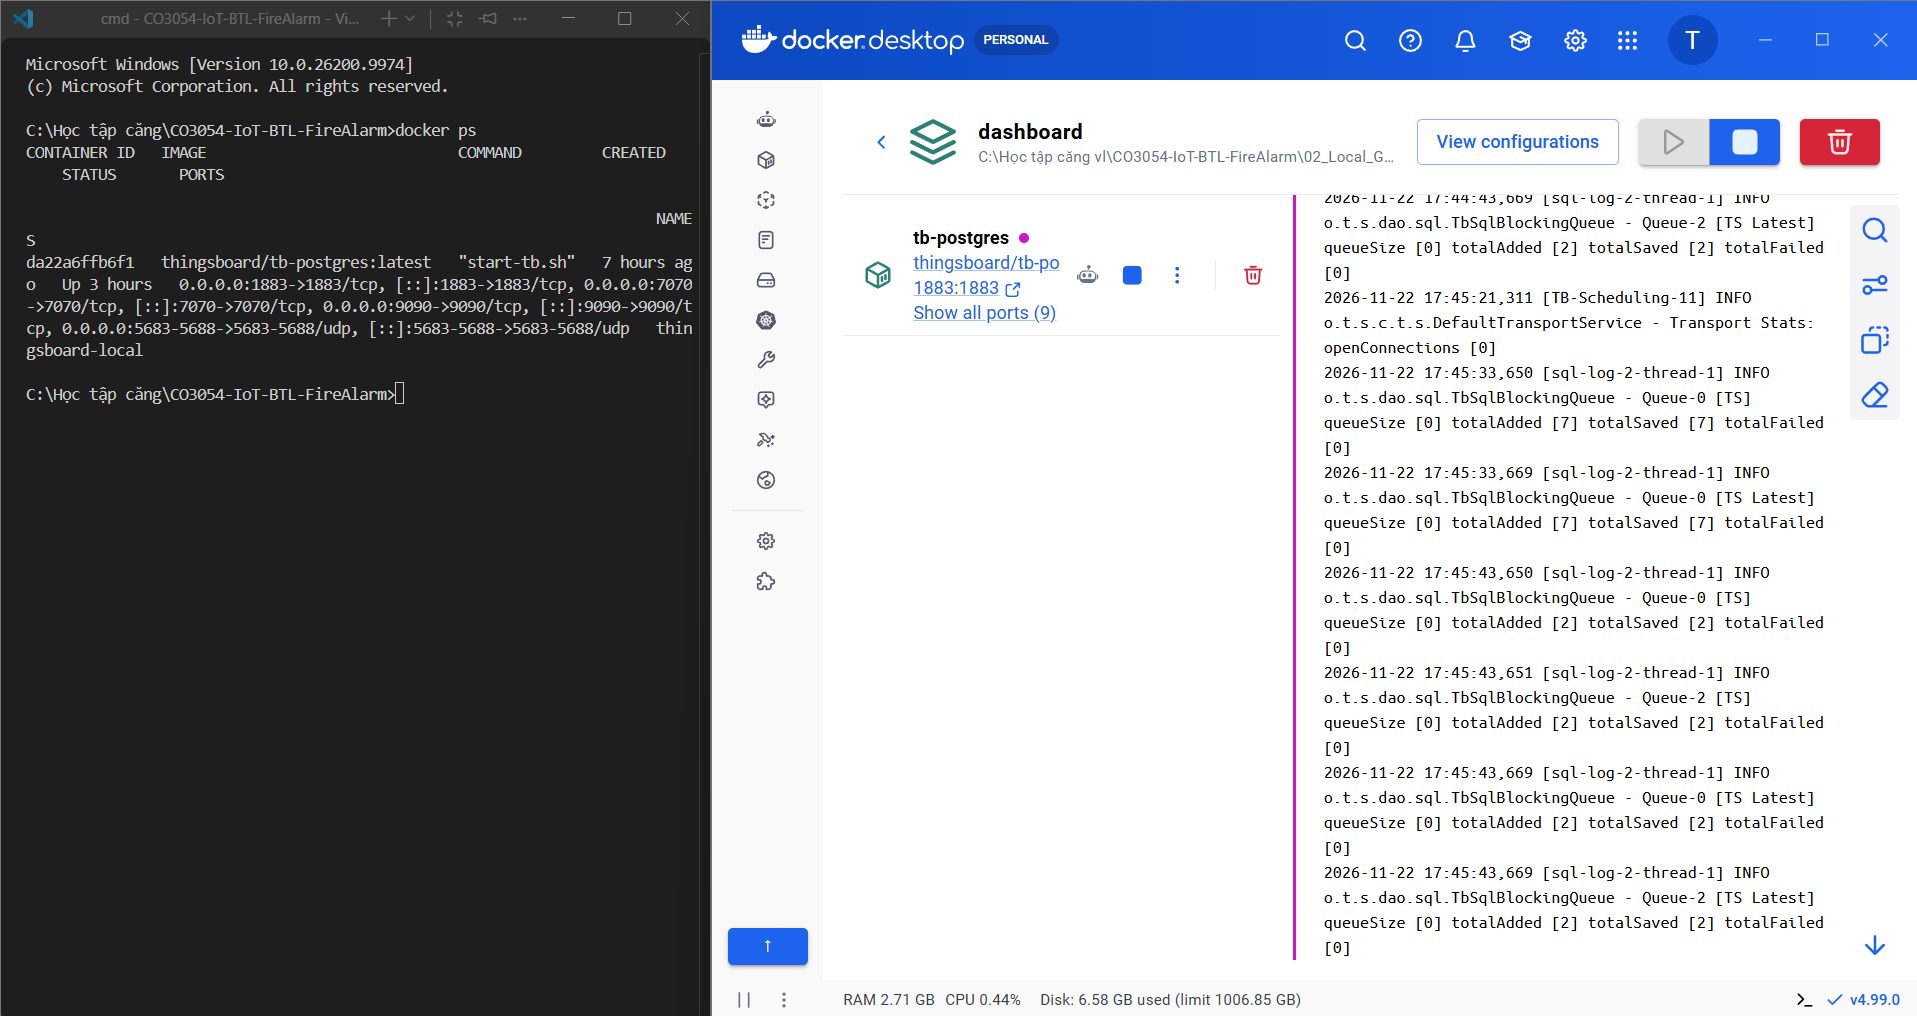
\includegraphics[width=0.92\textwidth]{../../captured_picture/N07.png}
  \caption{Container \texttt{thingsboard-local} chạy trên Docker Desktop với các cổng 9090 và 1883 (N07 -- \texttt{N07.png})}
  \label{fig:n07-docker}
\end{figure}
